\newif\ifsolutions
\solutionstrue % Show solutions
%\solutionsfalse % Hide solutions

\documentclass{article}
\usepackage{geometry}
\geometry{margin=1in}
\usepackage{tikz}
\usepackage{amssymb}

% fleqn allows setting indent of display math
\usepackage[fleqn]{amsmath}
\setlength{\mathindent}{0pt} % Set indent
% Disable equation numbering (https://tex.stackexchange.com/a/360378)
\makeatletter
\renewcommand\tagform@[1]{}
\makeatother

% Allow Unicode (some, e.g., © and £ at least)
% https://tex.stackexchange.com/questions/370278/is-there-any-reason-to-use-inputenc
\usepackage[utf8]{inputenc}

% Hyperlinks
\usepackage{hyperref}
\hypersetup{colorlinks=true, urlcolor=blue, linkcolor=blue}

% Prevent indentation of paragraphs
\setlength\parindent{0pt}
\setlength{\parskip}{\baselineskip}

% Spacing above/below equations
% https://tex.stackexchange.com/a/69678
\AtBeginDocument{%
 \abovedisplayskip=-\parskip
 \abovedisplayshortskip=-\parskip
 \belowdisplayskip=0pt
 \belowdisplayshortskip=0pt
}

% Allow 3 additional subsection levels
% https://tex.stackexchange.com/a/60212
\usepackage{titlesec}
\setcounter{secnumdepth}{6}
% H4 in HTML
\titleformat{\paragraph}{\normalfont\normalsize\bfseries}{\theparagraph}{1em}{}
\titlespacing*{\paragraph}{0pt}{3.25ex plus 1ex minus .2ex}{1.5ex plus .2ex}
% H5 in HTML
\titleformat{\subparagraph}{\normalfont\normalsize\bfseries}{\thesubparagraph}{1em}{}
\titlespacing*{\subparagraph}{0pt}{3.25ex plus 1ex minus .2ex}{1.5ex plus .2ex}
% H6 in HTML
\titleformat{\subsubparagraph}{\normalfont\normalsize\bfseries}{\thesubsubparagraph}{1em}{}
\titlespacing*{\subsubparagraph}{0pt}{3.25ex plus 1ex minus .2ex}{1.5ex plus .2ex}

% So enumerate at all levels is numbers
% https://tex.stackexchange.com/questions/78842/nested-enumeration-numbering
\renewcommand{\labelenumii}{\arabic{enumii}.}
\renewcommand{\labelenumiii}{\arabic{enumiii}.}
\renewcommand{\labelenumiv}{\arabic{enumiv}.}

\renewcommand{\mbox}{\text}
\newcommand{\ds}[0]{\displaystyle}
\newcommand{\ihat}[0]{\hat{\boldsymbol{\imath}}}
\newcommand{\jhat}[0]{\hat{\boldsymbol{\jmath}}}
\newcommand{\khat}[0]{\hat{\boldsymbol{k}}}
\newcommand{\xhat}[0]{\hat{\mathbf{x}}}
\newcommand{\yhat}[0]{\hat{\mathbf{y}}}
\newcommand{\zhat}[0]{\hat{\mathbf{z}}}
\newcommand{\rhat}[0]{\hat{\mathbf{r}}}
\newcommand{\bfvec}[1]{\vec{\mathbf{#1}}}
\newcommand{\bfcdot}[0]{\boldsymbol{\cdot}}

\usepackage{fancyhdr}
\pagestyle{fancy}
\lhead{The $\rhat$ Unit Vector}
\rhead{\thepage}
\fancyfoot{}

\begin{document}

% Figures:
% https://www.mathcha.io/editor/M55KMuQLiLmH9Vgp0Ptw6QGB3HnpzJnnuM6VoB7

\section{The $\rhat$ Unit Vector}

One approach to finding the electric force between two charges and the electric field due to a point charge is to use
$F=k{|q_1q_2|}/{r^2}$ to find the magnitude and a diagram to write $\bfvec{F}$ in the form $\bfvec{F}=F_x\ihat + F_y\jhat$.

An alternative approach is to use an equation for electric force and electric field using a unit vector $\rhat$. This approach is sometimes used for finding the electric field due to a continuous charge distribution. In addition, the $\rhat$ unit vector is often used when finding the magnetic field using the Biot--Savart law.

\subsection{Electric Force}

The equation for electric force (Coulomb's law) using a unit vector $\rhat$ is

$$\bfvec{F}_{q_1\text{ on }q_2}=kq_1q_2\frac{\rhat_{12}}{r^2}$$

where $\rhat_{12}$ is the unit vector that points from the position of $q_1$ to the position of $q_2$, and $r$ is the distance between $q_1$ and $q_2$.

To find $\rhat_{12}$,

\begin{enumerate}

  \item draw a vector, $\bfvec{r}_{12}$, from $q_1$ to $q_2$;

  \item Write $\bfvec{r}_{12}$ in the form $\bfvec{r}_{12}=r_x\ihat+r_y\jhat$ using the diagram; then

  \item $\rhat_{12}=\bfvec{r}_{12}/r$, where $r=\sqrt{r_x^2+r_y^2}$.

\end{enumerate}

\subsection{Electric Field}

The equation for electric field using a unit vector $\rhat$ is

$$\bfvec{E}_{\text{due to }q}=kq\frac{\rhat}{r^2}$$

where $\rhat$ is the unit vector that points from the position of $q$ to the point in space where we want to know $\bfvec{E}$, and $r$ is the distance between $q$ and that point. 

To find $\rhat$, 

\begin{enumerate}

  \item draw a vector, $\bfvec{r}$,from $q$ to the point in space where you want to know $\bfvec{E}$;

  \item Write $\bfvec{r}$ in the form $\bfvec{r}=r_x\ihat+r_y\jhat$ using the diagram; then

  \item $\rhat=\bfvec{r}/r$, where $r=\sqrt{r_x^2+r_y^2}$.

\end{enumerate}

Note that in the equations for $\bfvec{F}$ and $\bfvec{E}$, we do not need to take the absolute value of the charges.

\newpage

\section{Example I}

Charge $q_1$ is at $(x,y)=(-a,-a)$ and charge $q_2$ is at $(a, a)$. Find

\begin{enumerate}

  \item $\rhat_{12}$

  \item $\bfvec{F}_{q_1\text{ on }q_2}$

  \item $F_{q_1\text{ on }q_2}$

\end{enumerate}

\textbf{Solution}



\tikzset{every picture/.style={line width=0.75pt}} %set default line width to 0.75pt        

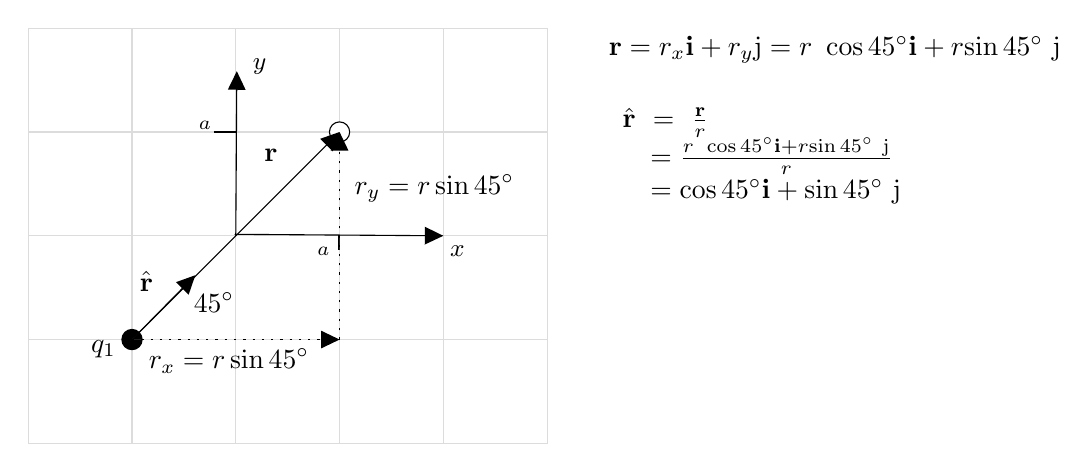
\begin{tikzpicture}[x=0.75pt,y=0.75pt,yscale=-1,xscale=1]
%uncomment if require: \path (0,227); %set diagram left start at 0, and has height of 227

%Shape: Grid [id:dp529276453314883] 
\draw  [draw opacity=0] (22.5,12) -- (272.5,12) -- (272.5,212) -- (22.5,212) -- cycle ; \draw  [color={rgb, 255:red, 220; green, 220; blue, 220 }  ,draw opacity=1 ] (72.5,12) -- (72.5,212)(122.5,12) -- (122.5,212)(172.5,12) -- (172.5,212)(222.5,12) -- (222.5,212) ; \draw  [color={rgb, 255:red, 220; green, 220; blue, 220 }  ,draw opacity=1 ] (22.5,62) -- (272.5,62)(22.5,112) -- (272.5,112)(22.5,162) -- (272.5,162) ; \draw  [color={rgb, 255:red, 220; green, 220; blue, 220 }  ,draw opacity=1 ] (22.5,12) -- (272.5,12) -- (272.5,212) -- (22.5,212) -- cycle ;
%Straight Lines [id:da9891788651841897] 
\draw    (122.5,112) -- (122.98,35.71) ;
\draw [shift={(123,32.71)}, rotate = 90.36] [fill={rgb, 255:red, 0; green, 0; blue, 0 }  ][line width=0.08]  [draw opacity=0] (8.93,-4.29) -- (0,0) -- (8.93,4.29) -- cycle    ;
%Straight Lines [id:da2531333242243323] 
\draw    (122,111.29) -- (219.5,111.98) ;
\draw [shift={(222.5,112)}, rotate = 180.41] [fill={rgb, 255:red, 0; green, 0; blue, 0 }  ][line width=0.08]  [draw opacity=0] (8.93,-4.29) -- (0,0) -- (8.93,4.29) -- cycle    ;
%Shape: Circle [id:dp928405560720714] 
\draw  [fill={rgb, 255:red, 0; green, 0; blue, 0 }  ,fill opacity=1 ] (67.63,162) .. controls (67.63,159.31) and (69.81,157.13) .. (72.5,157.13) .. controls (75.19,157.13) and (77.37,159.31) .. (77.37,162) .. controls (77.37,164.69) and (75.19,166.87) .. (72.5,166.87) .. controls (69.81,166.87) and (67.63,164.69) .. (67.63,162) -- cycle ;
%Shape: Circle [id:dp5390897406789283] 
\draw  [fill={rgb, 255:red, 255; green, 255; blue, 255 }  ,fill opacity=1 ] (167.63,62) .. controls (167.63,59.31) and (169.81,57.13) .. (172.5,57.13) .. controls (175.19,57.13) and (177.37,59.31) .. (177.37,62) .. controls (177.37,64.69) and (175.19,66.87) .. (172.5,66.87) .. controls (169.81,66.87) and (167.63,64.69) .. (167.63,62) -- cycle ;
%Straight Lines [id:da7315731890311423] 
\draw    (172.25,118.64) -- (172.25,111.64) ;
%Straight Lines [id:da41456511159458476] 
\draw    (112,62) -- (122.5,62) ;
%Straight Lines [id:da2368656312096422] 
\draw [fill={rgb, 255:red, 255; green, 255; blue, 255 }  ,fill opacity=1 ]   (72.5,162) -- (170.38,64.12) ;
\draw [shift={(172.5,62)}, rotate = 135] [fill={rgb, 255:red, 0; green, 0; blue, 0 }  ][line width=0.08]  [draw opacity=0] (8.93,-4.29) -- (0,0) -- (8.93,4.29) -- cycle    ;
%Straight Lines [id:da7182242007176092] 
\draw [fill={rgb, 255:red, 255; green, 255; blue, 255 }  ,fill opacity=1 ]   (72.5,162) -- (100.9,133.14) ;
\draw [shift={(103,131)}, rotate = 134.54] [fill={rgb, 255:red, 0; green, 0; blue, 0 }  ][line width=0.08]  [draw opacity=0] (8.93,-4.29) -- (0,0) -- (8.93,4.29) -- cycle    ;
%Straight Lines [id:da30412883702424365] 
\draw [fill={rgb, 255:red, 255; green, 255; blue, 255 }  ,fill opacity=1 ] [dash pattern={on 0.84pt off 2.51pt}]  (72.5,162) -- (169.5,162) ;
\draw [shift={(172.5,162)}, rotate = 180] [fill={rgb, 255:red, 0; green, 0; blue, 0 }  ][line width=0.08]  [draw opacity=0] (8.93,-4.29) -- (0,0) -- (8.93,4.29) -- cycle    ;
%Straight Lines [id:da8752471532648969] 
\draw [fill={rgb, 255:red, 255; green, 255; blue, 255 }  ,fill opacity=1 ] [dash pattern={on 0.84pt off 2.51pt}]  (172.5,162) -- (172.5,65) ;
\draw [shift={(172.5,62)}, rotate = 90] [fill={rgb, 255:red, 0; green, 0; blue, 0 }  ][line width=0.08]  [draw opacity=0] (8.93,-4.29) -- (0,0) -- (8.93,4.29) -- cycle    ;

% Text Node
\draw (129.5,25.4) node [anchor=north west][inner sep=0.75pt]  [font=\small]  {$y$};
% Text Node
\draw (224.5,115.4) node [anchor=north west][inner sep=0.75pt]  [font=\small]  {$x$};
% Text Node
\draw (160.5,116.4) node [anchor=north west][inner sep=0.75pt]  [font=\scriptsize]  {$a$};
% Text Node
\draw (103.5,55.4) node [anchor=north west][inner sep=0.75pt]  [font=\scriptsize]  {$a$};
% Text Node
\draw (135,69) node [anchor=north west][inner sep=0.75pt]   [align=left] {$\displaystyle \mathbf{r}$};
% Text Node
\draw (51.5,161) node [anchor=north west][inner sep=0.75pt]   [align=left] {$\displaystyle q_{1}$};
% Text Node
\draw (75,128) node [anchor=north west][inner sep=0.75pt]   [align=left] {$\displaystyle \hat{\mathbf{r}}$};
% Text Node
\draw (178.5,81) node [anchor=north west][inner sep=0.75pt]   [align=left] {$\displaystyle r_{y} =r\sin 45^{\circ }$};
% Text Node
\draw (79.37,165) node [anchor=north west][inner sep=0.75pt]   [align=left] {$\displaystyle r_{x} =r\sin 45^{\circ }$};
% Text Node
\draw (101,138) node [anchor=north west][inner sep=0.75pt]   [align=left] {$\displaystyle 45^{\circ }$};
% Text Node
\draw (301,47.4) node [anchor=north west][inner sep=0.75pt]    {$ \begin{array}{l}
\hat{\mathbf{r}} \ =\ \frac{\mathbf{r}}{r}\\
\ \ \ =\frac{r\ \cos 45\mathbf{^{\circ } i} +r\mathrm{\sin 45^{\circ } \ j}}{r}\\
\ \ \ =\cos 45\mathbf{^{\circ } i} +\mathrm{\sin 45^{\circ } \ j}
\end{array}$};
% Text Node
\draw (301,14.4) node [anchor=north west][inner sep=0.75pt]    {$\mathbf{r} =r_{x}\mathbf{i} +r_{y}\mathrm{j} =r\ \cos 45\mathbf{^{\circ } i} +r\mathrm{\sin 45^{\circ } \ j}$};


\end{tikzpicture}


The sides of the right triangle have length $2a$, so the hypotenuse $r=\sqrt{(2a)^2+(2a)^2}=\sqrt{8}a$. 

From the diagram, $\bfvec{r}_{12}=2a\ihat + 2a\jhat$, so $\ds\rhat_{12}=\frac{\bfvec{r}_{12}}{r}=\frac{1}{\sqrt{2}}\ihat + \frac{1}{\sqrt{2}}\jhat$

Note that the magnitude of $\rhat_{12}=1$: $|\rhat_{12}|=\sqrt{(1/2)^2+(1/2)^2}=1$

Substitution gives

$$\bfvec{F}_{q_1\text{ on }q_2}=kq_1q_2\frac{\rhat_{12}}{r^2} = \frac{kq_1q_2}{8a^2}\left[\frac{1}{\sqrt{2}}\ihat + \frac{1}{\sqrt{2}}\jhat\right]$$

Check: if $q_1$ and $q_2$ are both positive or both negative, the force on $q_2$ is upwards and to the right, as expected.

To calculate $|\bfvec{F}|$, we can use $|\bfvec{F}|=F=\sqrt{F_x^2+F_y^2}$ and plug in $F_x=k\frac{q_1q_2}{8a^2}\frac{1}{\sqrt{2}}$ and $F_y=k\frac{q_1q_2}{8a^2}\frac{1}{\sqrt{2}}$ and use $\sqrt{c^2}=|c|$ (where $c$ is a real number) to show that $F=k|q_1q_2|/{8a^2}$. There is an easier way. Taking the magnitude of both sides of

$\ds\bfvec{F}=kq_2q_1\frac{\rhat}{r^2}\quad$
gives
$\quad\ds|\bfvec{F}|=F=k|q_1q_2|\frac{|\rhat|}{r^2}$.

The magnitude of a unit vector is $1$, so
$\ds F=k|q_1q_2|\frac{1}{r^2}=k|q_1q_2|\frac{1}{8a^2}$.

\newpage

\section{Problem I}

Charge $q_1$ is at $(x,y)=(-a,a)$ and charge $q_2$ is at $(a, 0)$. Find

\begin{enumerate}

  \item $\rhat_{12}$

  \item $\bfvec{F}_{q_1\text{ on }q_2}$

  \item $F_{q_1\text{ on }q_2}$

\end{enumerate}

\ifsolutions
\textbf{Solution}

$r = \sqrt{5}a$

$\bfvec{r}_{12}=2a\ihat-a\jhat$

    \begin{enumerate}

      \item $\rhat_{12}=\bfvec{r}_{12}/r=\frac{2}{\sqrt{5}}\ihat-\frac{1}{\sqrt{5}}\jhat$

      \item $\ds\bfvec{F}_{q_1\text{ on }q_2}=kq_1q_2\frac{\rhat_{12}}{r^2}=\frac{kq_1q_2}{5a^2}\left(\frac{2}{\sqrt{5}}\ihat-\frac{1}{\sqrt{5}}\jhat\right)$

      \item $\ds F_{q_1\text{ on }q_2} = k|q_1q_2|\frac{1}{r^2}= k|q_1q_2|\frac{1}{5a^2}$

    \end{enumerate}
\else



\tikzset{every picture/.style={line width=0.75pt}} %set default line width to 0.75pt        

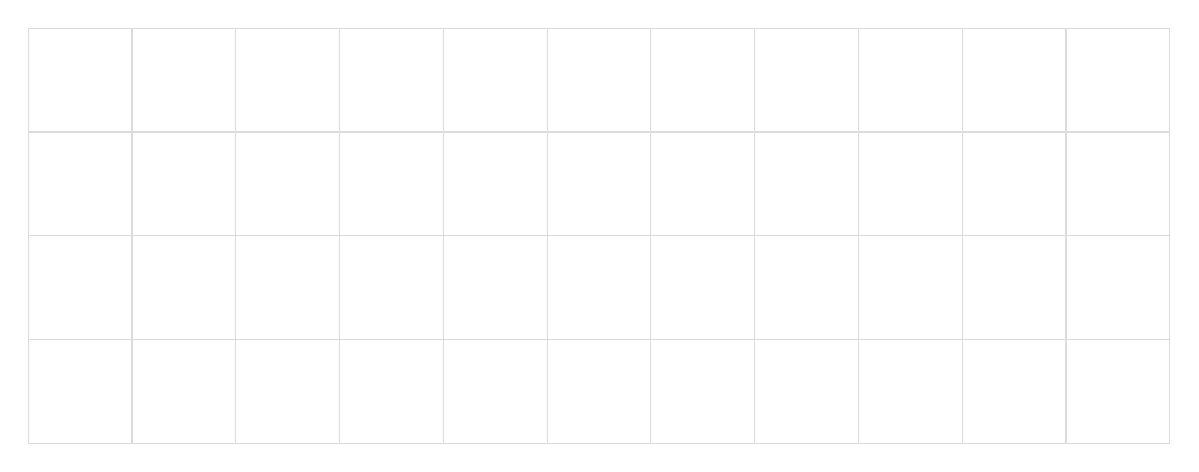
\begin{tikzpicture}[x=0.75pt,y=0.75pt,yscale=-1,xscale=1]
%uncomment if require: \path (0,208); %set diagram left start at 0, and has height of 208

%Shape: Grid [id:dp33505564538856114] 
\draw  [draw opacity=0] (2,2) -- (552,2) -- (552,202) -- (2,202) -- cycle ; \draw  [color={rgb, 255:red, 220; green, 220; blue, 220 }  ,draw opacity=1 ] (52,2) -- (52,202)(102,2) -- (102,202)(152,2) -- (152,202)(202,2) -- (202,202)(252,2) -- (252,202)(302,2) -- (302,202)(352,2) -- (352,202)(402,2) -- (402,202)(452,2) -- (452,202)(502,2) -- (502,202) ; \draw  [color={rgb, 255:red, 220; green, 220; blue, 220 }  ,draw opacity=1 ] (2,52) -- (552,52)(2,102) -- (552,102)(2,152) -- (552,152) ; \draw  [color={rgb, 255:red, 220; green, 220; blue, 220 }  ,draw opacity=1 ] (2,2) -- (552,2) -- (552,202) -- (2,202) -- cycle ;




\end{tikzpicture}

\fi

\newpage

\section{Example II}

If $q_1$ is at $(x,y)=(-a,-a)$, find

\begin{enumerate}

  \item $\rhat$

  \item $\bfvec{E}_{\text{at }(a,a)\text{ due to }q_1}$

  \item $E_{\text{at }(a,a)\text{ due to }q_1}$

\end{enumerate}

\textbf{Solution}

The calculation of $\rhat$ is the same as that shown in the diagram Example I (except we do not need subscripts for the $\bfvec{E}$ formula).

Substitution gives

$$\bfvec{E}_{\text{at }(a,a)\text{ due to }q_1}=kq_1\frac{\rhat}{r^2} =\frac{kq_1}{8a^2}\left[\frac{1}{\sqrt{2}}\ihat + \frac{1}{\sqrt{2}}\jhat\right]$$

Check: If a positive charge was placed at $(x,y)=(a,a)$, it would tend to move up and to the right, which is consitent with the signs on the components of the electric field found above.

To calculate $|\bfvec{E}|$, we can use

$$|\bfvec{E}|=E=\sqrt{E_x^2+E_y^2}$$

and plug in $E_x=k\frac{q_1}{8a^2}\frac{1}{\sqrt{2}}$ and $E_y=k\frac{q_1}{8a^2}\frac{1}{\sqrt{2}}$ and use $\sqrt{c^2}=|c|$ (where $c$ is a real number) to show that $E=k|q_1|/{8a^2}$. There is an easier way. Taking the magnitude of both sides of

$\ds\bfvec{E}=kq_1\frac{\rhat}{r^2}\quad$
gives
$\quad\ds|\bfvec{E}|=k|q_1|\frac{|\rhat|}{r^2}$.

The magnitude of a unit vector is $1$, so

$\ds|\bfvec{E}|=k|q_1|\frac{1}{r^2}=\frac{k|q_1|}{8a^2}$.

(Notice the relationship between the answers to this problem and the answers to Example I.)

\newpage

\section{Problem II}

If $q_1$ is at $(x,y)=(-a,a)$, find 

\begin{enumerate}

  \item $\rhat$

  \item $\bfvec{E}_{\text{at }(a,0)\text{ due to }q_1}$

  \item $E_{\text{at }(a,0)\text{ due to }q_1}$

\end{enumerate}

\ifsolutions
{\bf Solution}:

(Notice the relationship between the answers to this problem and the answers to Problem I.)

$r = \sqrt{5}a$

$\bfvec{r}_{12}=2a\ihat-a\jhat$

    \begin{enumerate}

      \item $\rhat_{12}=\bfvec{r}_{12}/r=\frac{2}{\sqrt{5}}\ihat-\frac{1}{\sqrt{5}}\jhat$

      \item $\ds\bfvec{E}=kq_1\frac{\rhat}{r^2}=\frac{kq_1}{5a^2}\left(\frac{2}{\sqrt{5}}\ihat-\frac{1}{\sqrt{5}}\jhat\right)$

      \item $\ds E = k|q_1|\frac{1}{r^2}= k|q_1|\frac{1}{5a^2}$

    \end{enumerate}
\else



\tikzset{every picture/.style={line width=0.75pt}} %set default line width to 0.75pt        

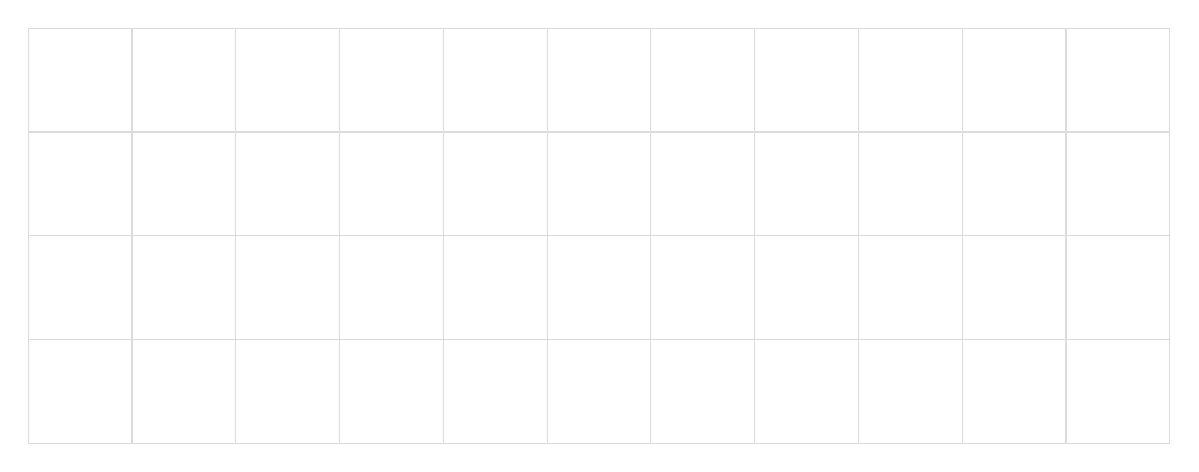
\begin{tikzpicture}[x=0.75pt,y=0.75pt,yscale=-1,xscale=1]
%uncomment if require: \path (0,208); %set diagram left start at 0, and has height of 208

%Shape: Grid [id:dp33505564538856114] 
\draw  [draw opacity=0] (2,2) -- (552,2) -- (552,202) -- (2,202) -- cycle ; \draw  [color={rgb, 255:red, 220; green, 220; blue, 220 }  ,draw opacity=1 ] (52,2) -- (52,202)(102,2) -- (102,202)(152,2) -- (152,202)(202,2) -- (202,202)(252,2) -- (252,202)(302,2) -- (302,202)(352,2) -- (352,202)(402,2) -- (402,202)(452,2) -- (452,202)(502,2) -- (502,202) ; \draw  [color={rgb, 255:red, 220; green, 220; blue, 220 }  ,draw opacity=1 ] (2,52) -- (552,52)(2,102) -- (552,102)(2,152) -- (552,152) ; \draw  [color={rgb, 255:red, 220; green, 220; blue, 220 }  ,draw opacity=1 ] (2,2) -- (552,2) -- (552,202) -- (2,202) -- cycle ;




\end{tikzpicture}

\fi

\newpage

\section{Additional Problems}

\subsection{Computing $\rhat$ for $\bfvec{F}$ formula}

If $q_1$ is at $(x,y)=(-a,2a)$ and $q_2$ is at $(x,y)=(a,0)$, find

\begin{enumerate}

  \item $\rhat_{12}$

  \item $\rhat_{21}$

  \item $r$

\end{enumerate}

\subsection{Computing $\rhat$ for $\bfvec{E}$ formula}

If $q_1$ is at $(x,y)=(a,0)$ and the point where we want to compute $\bfvec{E}$ is at $(x,y)=(-a,2a)$, find

\begin{enumerate}

  \item[2.] $\rhat$

  \item[3.] $r$

\end{enumerate}

\subsection{Finding $\rhat$ given positions in polar form}

Charge $q_1$ is a distance $a$ from the origin and at an angle of $45^\circ$ from the $+x$ axis (counterclockwise positive).

Charge $q_2$ is a distance $2a$ from the origin and at an angle of $135^\circ$ from the $+x$ axis (counterclockwise positive).

Find

\begin{enumerate}

  \item $\rhat_{12}$

  \item $\rhat_{21}$

\end{enumerate}

\subsection{Problem I Follow-up}

For the charge configuration given in Problem I, find

\begin{enumerate}

  \item $\rhat_{21}$

  \item $\bfvec{F}_{q_2\text{ on }q_1}$

  \item $F_{q_2\text{ on }q_1}$

\end{enumerate}

\end{document}